\vspace{-0.1in}
\section{Cost Analysis}
\label{sec:cost_model}

The adoption of switchless topology in data centers will probably be driven by the low-cost of such an architecture. In this section, we attempt to predict the cost of switchless in comparison to traditional architectures like conventional hierarchical and fat-tree. As an executive summary, the overhead cost per host for switchless was calculated to be around \$70, for conventional hierarchical between \$200 and \$2000, and for fat-tree between \$10000 and \$20000.

This section is organized into two subsections. First, we will state our assumptions of commodity equipments today, how they will look in short term future, and how that affect the cost equations. Second, we provide the cost equations themselves and a graph on the overhead cost vs. number of hosts in data centers.
\vspace{-0.1in}
\subsection{Assumptions}


\subsubsection{Commercial switches}

There are two types of switches utilized in our evaluations: a top-of-rack switch that has 36 10Gbps ports plus 4 uplink 40Gbps ports, and an aggregator switch that has 32 40Gbps ports. A quick survey reveals that the current cheapest price for these are \$7k and \$14k accordingly (Mellanox SX1012 and Mellanox SX1036).

\subsubsection{Interconnects}
First, we assumed a 10Gbps Ethernet connection on all hosts and switches, with the exception of hierarchical designs where top-of-rack and aggregators are using 40Gbps links.

Second, we assume that data centers will not use copper Ethernet for links longer than 15m. While at 10Gbps, certain copper connectors are rated at up to 100m, at 40Gbps this maximum length decreases to 30m, and while there is not yet a standard for 100Gbps copper Ethernet, we would guess that these will be only able to carry clean signal at an even shorter range. Therefore, while switchless can operate solely on copper Ethernet, other topologies will have to use fiber optics at the aggregation/core range. In the following cost equations, we do not take into account the copper cost, while the fiber optic link cost is assumed to be \$1 per meter, which requires a pair of optical transceivers (10GBASE-SR or 40GBASE-SR) each costing \$200.

\subsubsection{Costs related to switchless}
Integrating a network switch on-chip will incur cost in several areas of a microprocessor. We discuss a few of these: off-chip pins, power constraint, die area consumption, and external extension board for Ethernet jacks. While there can be many sources of on-chip network switch cost, silicon cost of an additional core and an extension board cost are two huge main factors. Other sources, such as additional off-chip pins, and thermal/power related costs are negligible. 
\newcommand{\subsubsubsection}{\textbf}

\subsubsubsection{Processor pins}
We do not think that off-chip pins requirement will be a significant factor in cost due to the low number of pins required for a Ethernet connection. A standard RJ45 Ethernet jack contains 4 differential-pairs, for a total of 8 pins. With a minimum of 6 ports required for a cube switchless topology, this means we need to dedicate 48 pins to the on-chip Ethernet switch. This is only 1.5x that of 32 pins requirement for a 16x PCI-E connection, of which a regular server has up to 40x. Furthermore, it is possible for Ethernet data to be transferred through PCI-E to get to the CPU.

\subsubsubsection{Power constraint}
As estimated in~\cite{cheapsilicon}, some reasonable power consumption per-link count for a 10Gbps switch is 1W for commodity switches, 3W for programmable pipelines, and 3W for general-purpose CPU-based switches. With 6 links for a cube topology, we would expect to spend 6-18W for power consumption, depending on implementation. While we do not include power consumption in our trade-off analysis, heat dissipation limit of the CPU is a major limitation on potential switchless architectures.

\subsubsubsection{Die area cost}
Die area cost of an on-chip switch is hugely dependent on the implementation, and the switching features needed. Here we will only give a bare minimum estimation.

The most favorable scenario for a minimum implementation is when we can have a custom routing protocol, like the dimension-ordered L3 protocol described in Section~\ref{sec:arch:sec:net_stack}. This implementation mirrors a router in a NoC: each host has its own unique XYZ coordinate, and a routing decision can be trivially made with a dimension comparison.

However, the same can be said for fat-tree or hierarchical topologies where a custom protocol can hugely improve performance and implementation cost. Instead, commercial switches need to adhere to standards like TCP, IP, and Ethernet, which complicate implementation. Assuming that we want our on-chip switch to be MAC address compatible, we would need to keep a MAC table big enough to store all the MACs in the immediate network. It turns out that such a 16k-entry table would be around 100KB in size. Furthermore, this table will need to be implemented as a hash-table, as CAMing a 16k-entry table is not feasible.

In the worst case, a dedicated CPU core is needed to manage the hash table. Now we have a different question: whether a single core is fast enough to switch packets without performance degradation. It turns out that, for 1500B packets and 10Gbps, an Ethernet link will interrupt the processor 833 times a second. A single RISC core at 2GHz will have ample time to multiplex multiple links.

Considering the cost of such a processor in products like Beaglebone, we estimate the silicon cost of an additional dedicated core at \$20 for calculation purposes.

\subsubsubsection{Extension board}
Hosts' motherboards will probably not have 6 Ethernet jacks to be used for switchless, so we include an extension board to the cost equation at \$50 per host.
\vspace{-0.1in}
\subsection{Cost model equations}
The general formula has three parts: the cost of switches, cost of interconnect (fiber optics), and other costs. This cost is "per-host".
\vspace{-0.1in}
\begin{multline}
Cost = Switch_{cost} + Interconnect_{cost} + Other_{cost}
\end{multline}
\subsubsection{Hierarchical}
In hierarchical topologies, we have three types of switches:
\vspace{-0.1in}
\begin{multline}
Switch_{cost} = ToR_{cost} + Agg_{cost} + Core_{cost}
\end{multline}
Top-of-rack switches are the low-end ones with 10Gbps connections to the hosts, and aggragators and core switches are assumed to be the same kind with 40Gbps ports.
\vspace{-0.1in}
\begin{multline}
Switch_{cost} = \$7000 * ToR_n +\\
                \$14000 * (Agg_n + Core_n)
\end{multline}
We assume that fiber optics are used to connect ToR, Agg, and Core together. The cost below includes the transceivers which cost \$200 each.
\vspace{-0.1in}
\begin{multline}
Interconnect_{cost} = \$450 * (ToR_n * Agg_n) +\\
                      \$500 * (Agg_n * Core_n)
\end{multline}
\subsubsection{Fat-tree}
The basic fat-tree for Ethernet as proposed in~\ref{fat-tree} has a $k$ parameter that dictates how many host the topology can support. It also utilizes only one type of switches. Fiber optics are assumed to be used between aggregation and core switches.
\vspace{-0.1in}
\begin{align}
Switch_{cost} = \$7000 * (K^2 + K^2 / 4) \\
Interconnect_{cost} = \$500 * (K^4 / 8)
\end{align}
\subsubsection{Switchless}
Switchless does not have switches, and we do not take into acount the copper Ethernet cables. Its other costs involve the cost of silicon (\$20) and the cost of the extension board (\$50).

\subsection{Analysis}

\captionsetup[subfloat]{captionskip=-0.003in}
\begin{figure}
    \centering
    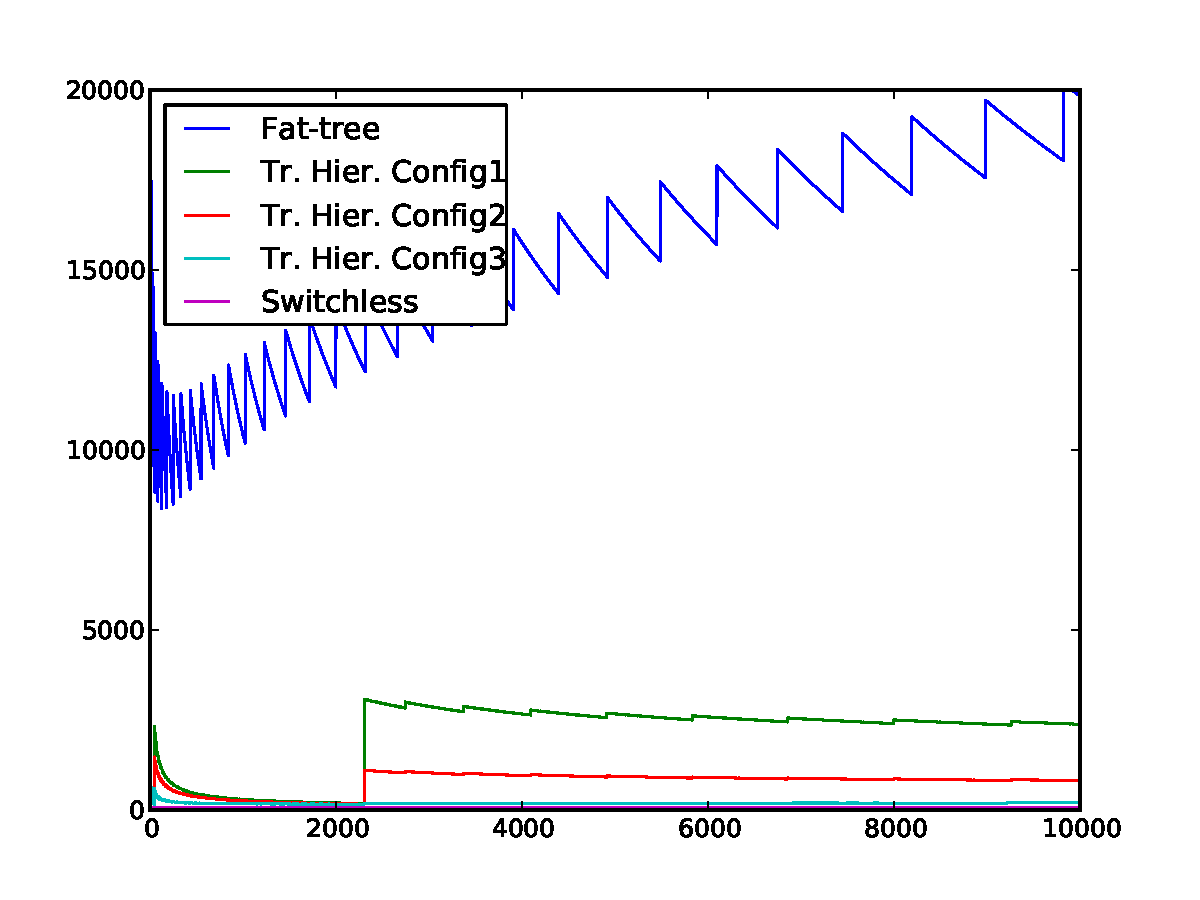
\includegraphics[width=0.3\textwidth]{10000_linear_permachinecost}
    \vspace{-0.1in}
    \caption{Per-host cost of network as number of host is increased to 10,000.}
    \label{fig:cost_perhost}
\end{figure}

As seen in Figure~\ref{fig:cost_perhost}, the cost of fat-tree can increase up to \$20000, traditional hierarchy (with bandwidth overprovisioning) to \$2000, while switchless remains a flat \$70.

